\documentclass[a4paper, 10pt, ]{article}

\usepackage[slovak]{babel}





\usepackage[utf8]{inputenc}
\usepackage[T1]{fontenc}

\usepackage[left=4cm,
			right=4cm,
            % left=2.5cm,
			% right=5.5cm,
			top=2.1cm,
			bottom=2.6cm,
			footskip=7.5mm,
			% twoside,
			marginparwidth=3.0cm,
			%showframe,
			]{geometry}

\usepackage{graphicx}
\usepackage[dvipsnames]{xcolor}
% https://en.wikibooks.org/wiki/LaTeX/Colors


% ------------------------------

\usepackage{lmodern}

\usepackage[tt={oldstyle=false,proportional=true,monowidth}]{cfr-lm}

% ------------------------------

\usepackage{amsmath}
\usepackage{amssymb}
\usepackage{amsthm}

\usepackage{booktabs}
\usepackage{multirow}
\usepackage{array}
\usepackage{dcolumn}


\usepackage[singlelinecheck=true]{subfig}


% ------------------------------


\def\naT{\mathsf{T}}

\hyphenpenalty=6000
\tolerance=1000




% ------------------------------


\makeatletter

	\def\@seccntformat#1{\protect\makebox[0pt][r]{\csname the#1\endcsname\hspace{4mm}}}

	\def\cleardoublepage{\clearpage\if@twoside \ifodd\c@page\else
	\hbox{}
	\vspace*{\fill}
	\begin{center}
	\phantom{}
	\end{center}
	\vspace{\fill}
	\thispagestyle{empty}
	\newpage
	\if@twocolumn\hbox{}\newpage\fi\fi\fi}

	\newcommand\figcaption{\def\@captype{figure}\caption}
	\newcommand\tabcaption{\def\@captype{table}\caption}

\makeatother


% ------------------------------




\usepackage{fancyhdr}
\fancypagestyle{plain}{%
\fancyhf{} % clear all header and footer fields
\fancyfoot[C]{\sffamily {\bfseries \thepage}\ | {\scriptsize\oznacenieCasti}}
\renewcommand{\headrulewidth}{0pt}
\renewcommand{\footrulewidth}{0pt}}
\pagestyle{plain}


% ------------------------------


\usepackage{titlesec}
\titleformat{\paragraph}[hang]{\sffamily  \bfseries}{}{0pt}{}
\titlespacing*{\paragraph}{0mm}{3mm}{1mm}
\titlespacing*{\subparagraph}{0mm}{3mm}{1mm}

\titleformat*{\section}{\sffamily\Large\bfseries}
\titleformat*{\subsection}{\sffamily\large\bfseries}
\titleformat*{\subsubsection}{\sffamily\normalsize\bfseries}






% ------------------------------

\PassOptionsToPackage{hyphens}{url}
\usepackage[pdfauthor={},
			pdftitle={},
			pdfsubject={},
			pdfkeywords={},
			% hidelinks,
			colorlinks=false,
			breaklinks,
			]{hyperref}


% ------------------------------


\graphicspath{%
{../fig_standalone/}%
{../../PY/fig/}%
{../../PY/jupynotex/fig/}%
{../../ML/fig/}%
{./fig/}%
}



% ------------------------------

\usepackage{enumitem}

\usepackage{lettrine}

% ------------------------------


\usepackage{microtype}


% ------------------------------

\usepackage[titles]{tocloft}

\setlength{\cftsecindent}{-12mm}
\setlength{\cftsecnumwidth}{12mm}
\renewcommand{\cftsecpresnum}{\hfill}
\renewcommand{\cftsecaftersnum}{\hspace{4mm}}

\setlength{\cftsubsecindent}{-12mm}
\setlength{\cftsubsecnumwidth}{16mm} % 12 + 4
\renewcommand{\cftsubsecpresnum}{\hfill}
\renewcommand{\cftsubsecaftersnum}{\hspace{8mm}} % 4 + 4 mm

\setlength{\cftsubsubsecindent}{-12mm}
\setlength{\cftsubsubsecnumwidth}{20mm} % 12 + 4 + 4
\renewcommand{\cftsubsubsecpresnum}{\hfill}
\renewcommand{\cftsubsubsecaftersnum}{\hspace{12mm}} % 4 + 4 + 4 mm

\renewcommand{\cftsecpagefont}{\lstyle \bfseries}
\renewcommand{\cftsubsecpagefont}{\lstyle}
\renewcommand{\cftsubsubsecpagefont}{\lstyle}



\setlength{\cftparaindent}{-16mm}
\setlength{\cftparanumwidth}{28mm} % 16 + 4 + 4 + 4
\renewcommand{\cftparapresnum}{\hfill}
\renewcommand{\cftparaaftersnum}{\hspace{16mm}} % 4 + 4 + 4 + 4 mm








% ------------------------------

\usepackage{listings}



\renewcommand{\lstlistingname}{Výpis kódu}
\renewcommand{\lstlistlistingname}{Výpisy kódu}




%New colors defined below
\definecolor{codegreen}{rgb}{0,0.6,0}
\definecolor{codegray}{rgb}{0.5,0.5,0.5}
\definecolor{codepurple}{rgb}{0.58,0,0.82}
\definecolor{backcolour}{rgb}{0.95,0.95,0.95}

%Code listing style named "mystyle"
\lstdefinestyle{mystyle}{
  backgroundcolor=\color{backcolour},
  commentstyle=\fontfamily{lmtt}\fontsize{8.5pt}{8.75pt}\selectfont\color{codegreen},
  keywordstyle=\fontfamily{lmtt}\fontsize{8.5pt}{8.75pt}\selectfont\bfseries\color{Blue},
  stringstyle=\fontfamily{lmtt}\fontsize{8.5pt}{8.75pt}\selectfont\color{codepurple},
  basicstyle=\fontfamily{lmtt}\fontsize{8.5pt}{8.75pt}\selectfont,
  breakatwhitespace=false,
  breaklines=true,
  captionpos=t,
  keepspaces=true,
  numbers=left,
  numbersep=4mm,
  numberstyle=\fontfamily{lmtt}\fontsize{8.5pt}{8.75pt}\selectfont\color{lightgray},
  showspaces=false,
  showstringspaces=false,
  showtabs=false,
  tabsize=2,
  % xleftmargin=10pt,
  framesep=10pt,
  language=Python,
  escapechar=|,
}


\lstset{
    inputencoding=utf8,
    extendedchars=true,
    literate=%
    {á}{{\'a}}1
    {č}{{\v{c}}}1
    {ď}{{\v{d}}}1
    {é}{{\'e}}1
    {ě}{{\v{e}}}1
    {í}{{\'i}}1
    {ň}{{\v{n}}}1
    {ó}{{\'o}}1
    {ř}{{\v{r}}}1
    {š}{{\v{s}}}1
    {ť}{{\v{t}}}1
    {ú}{{\'u}}1
    {ů}{{\r{u}}}1
    {ý}{{\'y}}1
    {ž}{{\v{z}}}1
    {Á}{{\'A}}1
    {Č}{{\v{C}}}1
    {Ď}{{\v{D}}}1
    {É}{{\'E}}1
    {Ě}{{\v{E}}}1
    {Í}{{\'I}}1
    {Ň}{{\v{N}}}1
    {Ó}{{\'O}}1
    {Ř}{{\v{R}}}1
    {Š}{{\v{S}}}1
    {Ť}{{\v{T}}}1
    {Ú}{{\'U}}1
    {Ů}{{\r{U}}}1
    {Ý}{{\'Y}}1
    {Ž}{{\v{Z}}}1
    {ô}{{\^{o}}}1
}


% ------------------------------


\usepackage{caption}

\DeclareCaptionFormat{odsadene}{\protect\makebox[0pt][r]{#1#2\hspace{4mm}}#3\par}
\DeclareCaptionLabelSeparator{lendvojbodka}{:}
% \DeclareCaptionFont{lightgray}{\color{lightgray}}
\DeclareCaptionFont{lightgray}{\fontfamily{lmtt}\fontsize{8.5pt}{8.75pt}\selectfont\color{lightgray}}

\captionsetup[lstlisting]{format=odsadene, labelsep=lendvojbodka, justification=raggedright, singlelinecheck=false, labelfont={sf, lightgray},}


% ------------------------------





% ------------------------------

\usepackage[backend=biber,
            style=numeric,
            sorting=none,
            ]{biblatex}
\DeclareSourcemap{
    \maps[datatype=bibtex]{
        \map{
        \step[fieldset=note, null]
        }
        \map{
        \step[fieldset=file, null]
        }        
        % \map{
        % \step[fieldset=url, null]        
        % }
        \map{
        \step[fieldset=eprint, null]
        }
    }
}


\addbibresource{E:/_CurrentContent/01_work_repo/bibLaTeXDB/bibLaTeXDB.bib} % nonpublic data





\def\oznacenieCasti{MRS05 - ZS2025}


\usepackage{longtable}




\begin{document}


\lstset{%
style=mystyle,
rangebeginprefix=\#\#\#\ cellB\ ,%
rangebeginsuffix=\ \#\#\#,%
rangeendprefix=\#\#\#\ cellE\ ,%
rangeendsuffix=\ \#\#\#,%
includerangemarker=false,
}





\fontsize{12pt}{22pt}\selectfont

\centerline{\textsf{Modelovanie a riadenie systémov} \hfill \textsf{\oznacenieCasti}}

\fontsize{18pt}{22pt}\selectfont





\begin{flushleft}
	\textbf{\textsf{Polprednáška o numerickom riešení diferenciálnych rovníc}}
\end{flushleft}





\normalsize

\bigskip

{\hypersetup{hidelinks}

\tableofcontents

}

\bigskip

\vspace{18pt}



\noindent
\lettrine[lines=3, nindent=0pt]{R}{iešením} diferenciálnej rovnice je funkcia času (v kontexte tohto textu), inými slovami časový priebeh veličiny, časová závislosť, signál. Túto funkciu času je vo všeobecnosti možné hľadať ako \emph{analytické riešenie}, teda na nájdenie matematického zápisu danej funkcie používame analytické postupy také, že výsledkom je matematický zápis či vyjadrenie danej funkcie. Inou možnosťou je hľadať \emph{numerické riešenie}, keď hľadáme postupnosť numerických hodnôt (čísiel), ktoré sú priradené k~časovým údajom tak, že je možné ukázať, že výslednú časovú postupnosť hodnôt je možné považovať za reprezentáciu funkcie času, ktorá je riešením dif. rovnice.












\section{ODE solver}


Pre hľadanie numerického riešenia sa využíva ODE solver\footnote{Solver je \emph{riešič}?  \emph{Riešidlo}?}. ODE je skratka pre obyčajné diferenciálne rovnice (ordinary differential equation).

Úlohou ODE solvera je nájsť numerické riešenie na základe rovnice (diferenciálnej), ktorú je možné vo všeobecnosti zapísať v tvare
\begin{equation} \label{fPreODESolver}
    \dot x(t) = f \left( t, x(t), \ldots \right)
\end{equation}
kde $f$ je funkcia, ktorej argumenty sú čas $t$, prirodzene, samotný výstupný (hľadaný, neznámy) signál $x(t)$ a prípadne iné ďalšie parametre či veličiny - napríklad externý vstup. Uvedená rovnica doslova predpisuje aká je časová zmena signálu $x(t)$. Časová zmena signálu, inými slovami časová derivácia (derivácia podľa času) je označená ako $\dot x(t)$.


\subsection{Numerická integrácia}

Ak teda do funkcie $f$ dosadíme hodnoty argumentov (čas, signál $x(t)$, a prípadne iné), získame hodnotu časovej zmeny $\dot x(t)$. Na základe informácie o $\dot x(t)$, ktorá zodpovedá aktuálnemu (dosadenému) signálu $x(t)$, môžeme určiť hodnotu $x(t)$ o~nejaký čas neskôr. Túto novú hodnotu $x(t)$ možno opäť dosadiť do funkcie $f$~a~následne nájsť ďalšiu ešte ďalej v čase - atď. ODE solver využíva práve tento jednoduchý princíp pre postupné hľadanie hodnôt (numerických hodnôt) signálu $x(t)$.


Vo všeobecnosti sa uvedený princíp nazýva numerická integrácia. ODE solver teda numericky integruje. Je množstvo metód pre numerickú integráciu, ktoré sa líšia spôsobom riešenia problémov súvisiacich so samotným procesom numerickej integrácie (voľba (optimalizácia) časového kroku integrácie, zohľadnenie matematických vlastností daného typu diferenciálnych rovníc a iné). ODE solvre sa môžu líšiť aj samotnou implementáciou niektorej z metód numerickej integrácie. Podrobnejší opis ODE solvera je nad rámec tohto textu.



\subsection{Zadefinovanie dynamického systému pre ODE solver}


\subsubsection{Schematické znázornenie dynamického systému}

Schematické znázornenie dynamického systému ako formu zadefinovania alebo naprogramovania dynamického systému pre ODE solver využíva napríklad softvér MATLAB - Simulink.

Pre zadefinovanie dynamického systému sa využívajú základné prvky -- bloky, ako zosilňovač, sumátor, integrátor a prípadne blok derivácie. Diferenciálnu rovnicu, ktorej numerické riešenie hľadáme, je v takomto prípade potrebné najskôr vyjadriť vo forme blokovej schémy.

\paragraph{Príklad s nehomogénnou rovnicou druhého rádu}

Uvažujme dynamický systém daný diferenciálnou rovnicou v tvare
\begin{equation} \label{eq:DR2R}
    \ddot y(t) + a_0 y(t) = b_0 u(t) \qquad y(0) = y_0, \quad \dot y(0) = z_0
\end{equation}
kde $y(t)$ je výstupný signál, $u(t)$ je vstupný signál, $a_0$ a $b_0$ sú konštantné parametre, $y_0$ a $z_0$ sú začiatočné podmienky. 

Rovnicu \eqref{eq:DR2R} prepíšme tak, aby na ľavej strane bola len najvyššia derivácia neznámej, teda signál $\ddot y(t)$
\begin{equation} \label{eq:DR2Rs}
    \ddot y(t)  = - a_0 y(t) + b_0 u(t) 
\end{equation}
Na začiatku máme k dispozícii signál $\ddot y(t)$, teda
\begin{center}

    \vbox{%
    \makebox[\textwidth][c]{%
    \input{../fig_standalone/schB_pr3_k1.pdf_tex}
    }

    \vspace{-30mm}

    \figcaption{Bloková schéma rovnice \eqref{eq:DR2Rs}, krok prvý.}
    \label{schB_pr3_k1.pdf}
    }

\end{center}
Signál $\ddot y(t)$ je v podstate súčtom dvoch iných signálov.
\begin{center}

    \vbox{%
    \makebox[\textwidth][c]{%
    \input{../fig_standalone/schB_pr3_k2.pdf_tex}
    }

    \vspace{-15mm}

    \figcaption{Bloková schéma rovnice \eqref{eq:DR2Rs}, krok druhý.}
    \label{schB_pr3_k2.pdf}
    }

\end{center}
Prvý signál získame zosilnením signálu $y(t)$ zosilňovačom so zosilnením $a_0$. Signál $y(t)$ je možné získať postupným integrovaním signálu $\ddot y(t)$.
\begin{center}

    \vbox{%
    \makebox[\textwidth][c]{%
    \input{../fig_standalone/schB_pr3_k3.pdf_tex}
    }

    \vspace{-15mm}

    \figcaption{Bloková schéma rovnice \eqref{eq:DR2Rs}, krok tretí.}
    \label{schB_pr3_k3.pdf}
    }

\end{center}
Druhý signál získame zosilnením známeho (dostupného) signálu $u(t)$ zosilňovačom so zosilnením $b_0$. 
\begin{center}

    \vbox{%
    \makebox[\textwidth][c]{%
    \input{../fig_standalone/schB_pr3_kf.pdf_tex}
    }

    \vspace{-15mm}    

    \figcaption{Bloková schéma rovnice \eqref{eq:DR2Rs}.}
    \label{schB_pr3_kf.pdf}
    }
\end{center}
Príslušné integrátori vo výslednej schéme musia mať začiatočné podmienky $y(0) = y_0$ a~$\dot y(0) = z_0$ (podľa \eqref{eq:DR2R}).










\subsubsection{Opis systému v stavovom priestore (sústava rovníc prvého rádu)}

Pre ODE solver, ktorý je implementovaný typicky ako funkcia v~programe, je v~podstate nevyhnutné zadefinovať dynamický systém vo forme zodpovedajúcej sústave diferenciálnych rovníc prvého rádu. Ako bolo uvedené v \eqref{fPreODESolver}, ODE solver tak bude mať k dispozícii funkciu dávajúcu do vzťahu stav systému a časovú zmenu stabu systému.

Hlavným krokom v takomto prípade teda je rozklad diferenciálnej rovnice vyššieho rádu na sústavu rovníc prvého rádu. Štandardným je postup zodpovedajúci postupnej derivácii (alebo integrácii z opačného hľadiska) keď východiskom je, že výstupná veličina systému je zároveň aj jednou zo stavových veličín systému.


\paragraph{Príklad s nehomogénnou rovnicou druhého rádu}

Uvažujme dynamický systém daný diferenciálnou rovnicou v tvare
\begin{equation} \label{eq:DR2R_2}
    \ddot y(t) + a_0 y(t) = b_0 u(t) \qquad y(0) = y_0, \quad \dot y(0) = z_0
\end{equation}
kde $y(t)$ je výstupný signál, $u(t)$ je vstupný signál, $a_0$ a $b_0$ sú konštantné parametre, $y_0$ a $z_0$ sú začiatočné podmienky. 

Ako prvé zvoľme
\begin{equation} \label{volba1}
    x_1(t) = y(t)
\end{equation}
To znamená
\begin{equation}
    \dot x_1(t) = \dot y(t)
\end{equation}
čo však nie je v tvare aký hľadáme. Na pravej strane vystupuje pôvodná veličina $y(t)$ a tu je cieľom mať sústavu rovníc kde vystupujú iba práve zavádzané stavové veličiny.

Druhou voľbou preto nech je
\begin{equation} \label{volba2}
    x_2(t) = \dot y(t)
\end{equation}
pretože potom môžeme písať prvú diferenciálnu rovnicu v tvare
\begin{equation}
    \dot x_1(t) = x_2(t)
\end{equation}
Ostáva zostaviť druhú diferenciálnu rovnicu. 

Keďže sme zvolili \eqref{volba2}, tak je zrejmé, že platí
\begin{equation} 
    \dot x_2(t) = \ddot y(t)
\end{equation}
Otázkou je $\ddot y(t) = \ ?$ Odpoveďou je pôvodná diferenciálna rovnica druhého rádu. Upravme \eqref{eq:DR2R_2} na tvar
\begin{align}
    \ddot y(t)  + a_0 y(t) &= b_0 u(t) \\
    \ddot y(t) &=  - a_0 y(t) +  b_0 u(t) 
\end{align}
To znamená, že
\begin{equation}  \label{druhadr_1}
    \dot x_2(t) =  - a_0 y(t) +  b_0 u(t) 
\end{equation}
čo však stále nie je požadovaný tvar druhej hľadanej diferenciálnej rovnice. Na pravej strane rovnice \eqref{druhadr_1} môžu figurovať len nové veličiny $x_1(t)$ a $x_2(t)$, nie pôvodná veličina $y(t)$. Stačí si však všimnúť skôr zvolené \eqref{volba1}. Potom môžeme písať
\begin{equation}  \label{druhadr_2}
    \dot x_2(t) =  - a_0 x_1(t) +  b_0 u(t) 
\end{equation}
čo je druhá hľadaná diferenciálna rovnica prvého rádu.

Diferenciálnu rovnicu druhého rádu \eqref{eq:DR2R_2} sme transformovali na sústavu diferenciálnych rovníc prvého rádu
\begin{subequations} \label{druhadr_sustava}
\begin{align}
    \dot x_1(t) &= x_2(t) \\
    \dot x_2(t) &=  - a_0 x_1(t) +  b_0 u(t) 
\end{align}
\end{subequations}

\subparagraph{Zápis v maticovom tvare:}

typicky sa pri dynamických systémoch hovorí o stavovom vektore, teda o vektore signálov, ktorého prvky sú stavové veličiny systému. 

V tomto príklade máme dve stavové veličiny, teda stavový vektor je
\begin{equation}
    x(t) = \begin{bmatrix} x_1(t) \\ x_2(t) \end{bmatrix}
\end{equation}
kde $x(t)$ ma teraz význam signálu, ktorý má dve zložky, dva prvky (azda dva kanály). Pre ODE solver je potrebné zadefinovať vzťah medzi stavovým vektorom a jeho časovou zmenou, teda vzťah medzi $x(t)$ a $\dot x(t)$. Signál $\dot x(t)$ je časová zmena stavového vektora, teda
\begin{equation}
    \dot x(t) = \begin{bmatrix} \dot x_1(t) \\ \dot x_2(t) \end{bmatrix}
\end{equation}

Na základe \eqref{druhadr_sustava} môžeme písať
\begin{equation}
    \dot x(t) = \begin{bmatrix} \dot x_1(t) \\ \dot x_2(t) \end{bmatrix} = \begin{bmatrix} x_2(t) \\ - a_0 x_1(t) +  b_0 u(t) \end{bmatrix}
\end{equation}
Aby bol zrejmý vzťah medzi $x(t)$ a $\dot x(t)$, je potrebné vyňať stavový vektor $x(t)$, teda 
\begin{equation}
     \begin{bmatrix} \dot x_1(t) \\ \dot x_2(t) \end{bmatrix} = \begin{bmatrix} 0 & 1 \\ -a_0 & 0 \end{bmatrix} \begin{bmatrix} x_1(t) \\ x_2(t) \end{bmatrix} + \begin{bmatrix} 0 \\ b_0 \end{bmatrix} u(t)
\end{equation}
Tým vznikli matica 
\begin{equation}
    A = \begin{bmatrix} 0 & 1 \\ -a_0 & 0 \end{bmatrix}
\end{equation}
a vektor
\begin{equation}
    b = \begin{bmatrix} 0 \\ b_0 \end{bmatrix}
\end{equation}
Systém zapísaný v maticovom tvare teda je
\begin{equation} \label{stavovyPriestorPriklad}
    \dot x(t) = Ax(t) + bu(t)   
\end{equation}

Je možné pridať aj tzv. výstupnú rovnicu, ktorá dáva do vzťahu stavový vektor a~výstupný signál systému. V tomto prípade je výstupný signál $y(t)$ rovný prvej stavovej veličine $x_1(t)$, teda
\begin{equation}
    y(t) = \begin{bmatrix} 1 & 0 \end{bmatrix} \begin{bmatrix} x_1(t) \\ x_2(t) \end{bmatrix}
\end{equation}
kde sme zaviedli vektor 
\begin{equation}
    c = \begin{bmatrix} 1 \\ 0 \end{bmatrix}
\end{equation}

Pre úplnosť napíšme celý systém v stavovom opise
\begin{subequations} \label{stavovyPriestorPrikladCely}
\begin{align}
    \dot x(t) &= Ax(t) + bu(t)   \\
    y(t) &= c^\naT  x(t)
\end{align}
\end{subequations}









\section{Kyvadlo ako príklad dynamického systému\newline pre hľadanie numerického riešenia}


Uvažujme kyvadlo, ktorého kmity sú tlmené viskóznym trením s~koeficientom $\beta$ [kg~m$^2$~s$^{-1}$]. Kyvadlo je na Obr.~\ref{Kyvadlo}, kde hmotný bod s~hmotnosťou $m$ [kg] pripevnený na ramene so zanedbateľnou hmotnosťou a~dĺžkou $l$ [m] kmitá, $o$~označuje os otáčania kolmú na rovinu, v~ktorej kyvadlo kmitá, uhol medzi zvislicou a~ramenom kyvadla je označený $\varphi$ [rad] a~gravitačné zrýchlenie $g$~[m~s$^{-2}$].
\begin{center}

    \vbox{%
	\makebox[\textwidth][c]{%
	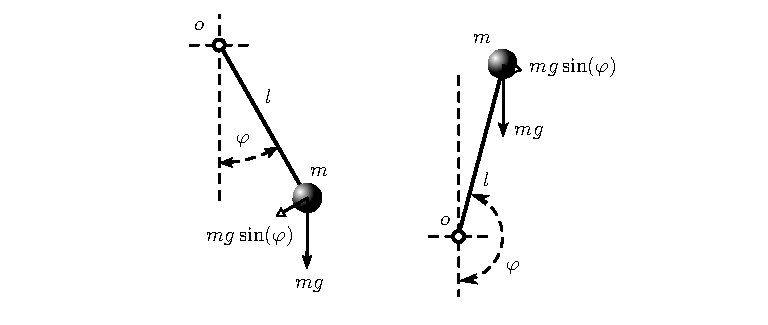
\includegraphics{Obr_Kyvadlo.pdf}
	}
	\vspace{-9mm}

	\figcaption{Kyvadlo}
	\label{Kyvadlo}
    }

	\vspace{-3mm}
\end{center}
Pohybová rovnica opisujúca dynamiku rotačného pohybu kyvadla je v tvare
\begin{subequations} \label{PohRovKyvadla}
\begin{align}
		&ml^2 \ddot{\varphi}(t) + \beta \dot{\varphi}(t) + mgl\sin{\left(\varphi(t)\right)} = u(t) \label{PohRovKyvadlab} \\
		&ml^2 \ddot{\varphi}(t) = -\beta \dot{\varphi}(t) - mgl\sin{\left(\varphi(t)\right)} + u(t)
\end{align}
\end{subequations}
kde $u(t)$ [kg~m$^2$~s$^{-2}$] je externý moment sily pôsobiaci na rameno kyvadla, $\dot{\varphi}(t)$ [rad~s$^{-1}$] je uhlová rýchlosť a~$\ddot{\varphi}(t)$~[rad~s$^{-2}$] je uhlové zrýchlenie ramena kyvadla. Číselné hodnoty parametrov kyvadla sú uvedené v tabuľke~\ref{Parametre kyvadla}.
\begin{center}

    \vbox{
    
    \tabcaption{Parametre kyvadla}
    \label{Parametre kyvadla}
    
    \vspace{-3mm}
    
    \begin{tabular*}{\textwidth}{ c @{\extracolsep{\fill}} c c}
        
        \toprule
        Parameter   & Hodnota    & Jednotky              \\
        \midrule
        $m$       & $1$   & kg             \\
        $l$    &  $1$  & m \\
        $g$   & $9,81$  & m s$^{-2}$ \\
        $\beta$  &  $2 \cdot 0,5 \cdot \sqrt{g/l}$ &  kg~m$^2$~s$^{-1}$ \\
        \bottomrule\
    
    \end{tabular*}
    } 
    
    \vspace{-3mm}
    
\end{center}


\subsection{Model dynamického systému}

Rovnica \eqref{PohRovKyvadla} je modelom uvažovaného dynamického systému. Model je matematická reprezentácia v tomto prípade fyzikálneho systému. Model umožňuje uvažovať o~systéme a~predpovedať ako sa bude systém správať.

\subsubsection{Vstupno-výstupný model systému}
    
Uvedený model opisuje vstupno-výstupné správanie sa dynamického systému, kde vstupom je externý moment sily $u(t)$ a~výstupom je uhol $\varphi(t)$, avšak budeme pracovať aj opisom systému v~\uv{stavovom priestore}.


\subsubsection{Opis systému v stavovom priestore}

Stav systému je súbor premenných (súbor veličín), ktoré sumarizujú minulosť systému pre potreby predpovede budúcnosti systému. Pre fyzikálny systém je stav zložený z~premenných potrebných pre výpočet zmeny hmotnosti, hybnosti a energie. Kľúčovou otázkou pri vytváraní modelu je ako presne má byť táto zmena popísaná.

Stavové premenné tvoria vektor $x(t) \in  \mathbb{R}^n$, ktorý sa nazýva \emph{stavový vektor}. Vstupy, pomocou ktorých je systém riadený, tvoria vektor vstupov $u(t) \in \mathbb{R}^p$ a~merateľné výstupy systému tvoria vektor výstupov $y(t) \in \mathbb{R}^q$. V~tomto prípade máme $p = q = 1$. Dynamický systém  potom možno reprezentovať rovnicami v~tvare
\begin{subequations} \label{GeneralLTIsyst}
\begin{align}
	\dot{x}(t) &= f(x(t),u(t)) \\
	y(t) &= h(x(t),u(t))
\end{align}
\end{subequations}
kde $f: \mathbb{R}^n \times \mathbb{R}^p \rightarrow \mathbb{R}^n$ a~$h: \mathbb{R}^n \times \mathbb{R}^p \rightarrow \mathbb{R}^q$ sú hladké funkcie. Model v takomto tvare nazývame \emph{model v~stavovom priestore}.

Rozmer stavového vektora sa nazýva \emph{rád systému}. Systém \eqref{GeneralLTIsyst} sa nazýva \emph{časovo-invariantný} pretože funkcie $f$ a $h$ nie sú priamo závislé na čase $t$. Pri časovo-variantných systémoch sú. Model pozostáva z~dvoch funkcií: funkcia $f$ určuje rýchlosť zmeny stavového vektora ako funkciu stavu $x(t)$~a~vstupu $u(t)$, a~funkcia $h$~určuje merateľné výstupy ako funkciu stavu $x(t)$ a vstupu $u(t)$.



\paragraph{Lineárny systém}

Systém sa nazýva lineárny ak sú funkcie $f$~a~$h$~lineárne vzhľadom na $x$~a~$u$. Lineárny model v stavovom priestore má tvar
\begin{subequations} \label{LinearLTIsyst}
\begin{align}
	\dot x(t) &= Ax(t) + Bu(t) \\
	y(t) &= Cx(t) + Du(t)
\end{align}
\end{subequations}
kde $A$, $B$, $C$ a $D$ sú konštantné matice. Takýto systém sa nazýva lineárny a časovo-invariantný, v skratke LTI z anglického linear and time-invariant. Matica $A$ sa nazýva dynamická matica, matica $B$ sa nazýva vstupná matica, matica $C$ sa nazýva výstupná matica a matica $D$ sa nazýva priamy člen. Drvivá väčšina systémov nemá priamy člen, čo znamená, že vstup nemá priamy vplyv na výstup.

Lineárny dynamický systém je možné zapísať v tvare lineárnej obyčajnej diferenciálnej rovnice
\begin{align} \label{vseobDifRov}
	\frac{\text{d}^n y(t)}{\text{d}t^n} + a_{n-1} \frac{\text{d}^{(n-1)} y(t)}{\text{d}t^{(n-1)}} + \cdots + a_0 y(t) = b_0 u(t)
\end{align}
kde $t$ je nezávisle premenná (čas), $y(t)$ je závisle premenná (výstup) a $u(t)$ je vstup. Zápis $\frac{\text{d}^n y}{\text{d}t^n}$ značí $n$-tú deriváciu $y(t)$ podľa času $t$. Hovoríme, že rovnica \eqref{vseobDifRov} je diferenciálna rovnica $n$-tého rádu, ktorá modeluje dynamiku systému $n$-tého rádu. Konverzia na model v stavovom priestore je napríklad definovaním stavového vektora v~tvare
\begin{align}
	x(t)
	=
	\begin{bmatrix}
		x_1(t) \\ x_2(t) \\ \vdots \\ x_n
	\end{bmatrix}
	=
	\begin{bmatrix}
		y(t) \\ \frac{\text{d}y(t)}{\text{d}t} \\ \vdots \\ \frac{\text{d}^{(n-1)} y(t)}{\text{d}t^{(n-1)}}
	\end{bmatrix}
\end{align}
potom model v stavovom priestore možno zapísať v~tvare
\begin{subequations}
\begin{align}
	\frac{\text{d}}{\text{d}t}
	\begin{bmatrix}
		x_1(t) \\ x_2(t) \\ \vdots \\ x_n(t)
	\end{bmatrix}
	&=
	\begin{bmatrix}
		x_{n-1}(t) \\ x_{n-2}(t) \\ \vdots \\ -a_{n-1} x_n(t) - \cdots - a_0 x_1(t)
	\end{bmatrix}
	+
	\begin{bmatrix}
		0 \\ 0 \\ \vdots \\ b_0 u(t)
	\end{bmatrix}
	\\
	y(t) &= x_1(t)
\end{align}
\end{subequations}
čo po vhodnej definícii matíc $A$, $B$, $C$ a $D$ má tvar \eqref{LinearLTIsyst}. Napríklad je možné, že výstup bude lineárnou kombináciou všetkých stavových veličín (predpokladáme, že výstup nezávisí priamo od vstupu), teda
\begin{align}
	y(t) = c_1 x_1(t) + c_2 x_2(t) + \cdots + c_n x_n(t)
\end{align}
Potom model v stavovom priestore je
\begin{subequations}
\begin{align}
%\begin{split}
	\dot{x}(t)
	&
	=
	%&
	\begin{bmatrix}
  	0      & 1      & 0      & \cdots & 0      & 0      \\
   	0      & 0      & 1      & \ddots & 0      & 0      \\
    \vdots & \vdots & \ddots & \ddots & \ddots & \vdots \\
    0      & 0      & 0      & \ddots & 1      & 0      \\
    0      & 0      & 0      & \cdots & 0      & 1      \\
   	-a_0   & -a_1   & -a_2   & \cdots &-a_{n-2}&-a_{n-1}
	\end{bmatrix}
	\begin{bmatrix}
		x_1(t) \\ x_2(t) \\ \vdots \\ x_{n-2}(t) \\x_{n-1}(t)  \\ x_n(t)
	\end{bmatrix} +
	%&
	\begin{bmatrix}
		0 \\ 0 \\ \vdots \\ 0 \\0  \\ b_0
	\end{bmatrix}
	u(t)
%\end{split}
\\
y(t) &= \begin{bmatrix}
		c_1& c_2 & \hdots & c_{n-2} & c_{n-1}  &c_n
	\end{bmatrix}
	x(t)
\end{align}
\end{subequations}





\paragraph{Nelineárny systém}

Máme rovnicu opisujúcu dynamiku rotačného pohybu kyvadla. Rovnica je v tvare
\begin{equation}
    ml^2 \ddot{\varphi}(t) + \beta \dot{\varphi}(t) + mgl\sin{\left(\varphi(t)\right)} = u(t)
\end{equation}
Túto rovnicu (rovnicu \eqref{PohRovKyvadlab}) možno prepísať aj na tvar
\begin{align}
	\ddot{\varphi}(t) = - \frac{\beta}{ml^2} \dot{\varphi}(t) - \frac{g}{l} \sin\left(\varphi(t)\right) + \frac{1}{ml^2}u(t)
\end{align}
čo je v tomto prípade úprava len kozmetická, ale relatívne užitočná, ako sa ukáže.


Každú diferenciálnu rovnicu vyššieho rádu je možné zapísať ako sústavu rovníc prvého rádu. Napríklad sústavu dvoch rovníc prvého rádu je možné vo všeobecnosti zapísať v tvare
\begin{equation} \label{naznak01}
   \begin{bmatrix} \dot x_1(t) \\ \dot x_2(t) \end{bmatrix} = F \left( t, \begin{bmatrix} x_1(t) \\ x_2(t) \end{bmatrix}, \ldots \right)
\end{equation}


V takejto novej sústave rovníc, vo všeobecnosti, vznikli nové veličiny (signály), ktoré sa vo všeobecnosti môžu líšiť od pôvodných veličín (signálov) v pôvodnej rovnici vyššieho rádu.

Nové veličiny vystupujúce v sústave rovníc sa v teórii systémov súhrnne označujú ako stav systému (stavové veličiny systému). Ak poznáme aktuálny stav systému potom spravidla vieme určiť predchádzajúce aj budúce stavy (vo všeobecnosti).

Napr. v rovnici kyvadla vystupujú veličiny (signály) $\ddot \varphi(t)$, $\dot \varphi(t)$ a~$\varphi(t)$. Je zrejmé (možno nie nad slnko jasné), že ako stav systému je možné zvoliť veličiny $\varphi(t)$ a $\dot \varphi(t)$, teda polohu a~uhlovú rýchlosť kyvadla. Ak poznáme tieto, poznáme celú históriu a~budúcnosť pohybu kyvadla.

Môže existovať viac možností voľby stavových veličín. Pri lineárnych systémoch je možností nekonečne veľa (nekonečne veľa stavových priestorov). Z praktického hľadiska však majú význam len niektoré voľby - napr. pri pohybových systémoch, akým je kyvadlo, sú to prirodzene poloha, rýchlosť, zrýchlenie, trh atď., v~závislosti od rádu systému.


Jednou z možností ako previesť rovnicu vyššieho rádu na sústavu rovníc prvého rádu je nasledovný postup. V tomto prípade je zhodou okolností výsledkom aj prakticky využiteľný stavový priestor (stavové veličiny $\varphi(t)$ a $\dot \varphi(t)$). Nech
\begin{equation}
    x_1(t) = \varphi(t)
\end{equation}
potom
\begin{equation}
    \dot x_1(t) = \dot \varphi(t)
\end{equation}
Ďalej nech
\begin{equation}
    \dot x_1(t) = \dot \varphi(t) = x_2(t)
\end{equation}
a to znamená, že
\begin{equation}
    \dot x_2(t) = \ddot \varphi(t)
\end{equation}
Tým sme získali veličiny $x_1(t) = \varphi(t)$ a $x_2(t) = \dot \varphi(t)$. Je možné zostaviť stavový vektor $x = \begin{bmatrix} x_1(t) & x_2(t) \end{bmatrix}^\mathsf T$ a teda $\dot x = \begin{bmatrix} \dot x_1(t) & \dot x_2(t) \end{bmatrix}^\mathsf T$.

Ako sme naznačili v súvislosti s \eqref{naznak01}, cieľom je vlastne konkretizovať funkciu $F$ v~rovnici
\begin{equation}
    \dot x = F(t, x, \ldots)
\end{equation}
čo je kompaktný zápis sústavy
\begin{align}
    \dot x_1(t) &= F_1 \left(t, x_1(t), x_2(t), \ldots \right) \\
    \dot x_2(t) &= F_2 \left(t, x_1(t), x_2(t), \ldots \right)
\end{align}

Prvú rovnicu v tomto prípade máme:
\begin{equation}
    \dot x_1(t) = x_2(t)
\end{equation}
Druhá rovnica vyplynie z postrehu, že pôvodnú rovnicu druhého rádu možno zapísať v tvare
\begin{align}
    \begin{split}
    \ddot \varphi(t) &= -\frac{\beta}{ml^2}\dot\varphi(t) - \frac{g}{l} \sin\left( \varphi(t) \right) + \frac{1}{ml^2} u(t) \\
                     &= -\frac{\beta}{ml^2} x_2(t) - \frac{g}{l} \sin\left( x_1(t) \right) + \frac{1}{ml^2} u(t)
    \end{split}
\end{align}
kde sú využité novo zavedené stavové veličiny $x_1(t)$ a $x_2(t)$. Je zrejmé, že druhá rovnica sústavy je
\begin{equation}
    \dot x_2(t) = -\frac{\beta}{ml^2} x_2(t) - \frac{g}{l} \sin\left( x_1(t) \right) + \frac{1}{ml^2} u(t)
\end{equation}
a teda rovnice kyvadla v stavovom priestore sú
\begin{align} \label{rovniceKyvSSpredpis}
    \begin{bmatrix} \dot x_1(t) \\ \dot x_2(t)  \end{bmatrix} = \begin{bmatrix} x_2(t) \\ -\frac{\beta}{ml^2} x_2(t) - \frac{g}{l} \sin\left( x_1(t) \right)  \end{bmatrix} + \begin{bmatrix} 0 \\ \frac{1}{ml^2} \end{bmatrix} u(t)
\end{align}
čím je funkcia $F$ jasne stanovená.

Stavom kyvadla sú dve veličiny: uhol natočenia ramena kyvadla $\varphi(t)$ a~uhlová rýchlosť ramena kyvadla $\dot\varphi(t)$. Stavový vektor má preto dva prvky $x^{\mathsf{T}}(t) = \begin{bmatrix} x_1(t) & x_2(t)	\end{bmatrix}$, kde $x_1(t) = \varphi(t)$ a~$x_2(t) = \dot\varphi(t)$. Model kyvadla v stavovom priestore je v tvare
\begin{subequations}
	\begin{align}
		\begin{bmatrix}
			\dot{x}_1(t) \\ \dot{x}_2(t)
		\end{bmatrix}
		&=
		\begin{bmatrix}
			x_2(t) \\ - \frac{\beta}{ml^2} x_2(t) - \frac{g}{l} \sin(x_1(t))
		\end{bmatrix}
		+
		\begin{bmatrix}
			0 \\ \frac{1}{ml^2}
		\end{bmatrix}
		u(t) \\
		\varphi(t) &= x_1(t)
	\end{align}
\end{subequations}
Toto je nelineárny časovo-invariantný systém druhého rádu.







\section{Používanie ODE solvera}

ODE solver ako funkcia v programe môže mať napríklad nasledujúce vstupy (argumenty) a výstupy:

\begin{verbatim}
x = odesolver(fcnF, init, timeVect)
\end{verbatim}
kde \verb|x| je, samozrejme, hľadané numerické riešenie. Prvým argumentom je funkcia s~názvom \verb|fcnF|, ktorá implementuje sústavu diferenciálnych rovníc v zmysle predchádzajúceho textu. \verb|init| označuje začiatočné hodnoty stavových veličín. \verb|timeVect| označuje časové okamihy (vzorky), v ktorých hľadáme hodnoty numerického riešenia.



\subsection{MATLAB}


MATLAB obsahuje hneď niekoľko ODE solverov. Tu budeme používať \verb|ode45|.


\paragraph{Autonómny systém (bez vstupného signálu)}

Vytvorme funkciu, ktorá realizuje sústavu diferenciálnych rovníc \eqref{rovniceKyvSSpredpis}, avšak, uvažujme, že vstupný signál $u(t)$ je nulový. Teda neuvažujme vstupný signál vôbec. Ešte inými slovami, externý moment sily je nulový, $u(t) = 0$ a preto potom možno písať
\begin{align} \label{fajnVektRov0}
	\begin{bmatrix}
		\dot{x}_1 \\ \dot{x}_2
	\end{bmatrix}
	&=
	\begin{bmatrix}
		x_2 \\ - \frac{\beta}{ml^2} x_2 - \frac{g}{l} \sin(x_1)
	\end{bmatrix}
\end{align}
Toto je autonómny nelineárny časovo-invariantný systém druhého rádu. Jeho správanie závisí len od začiatočného stavu na začiatku uvažovaného času.

Funkcia, ktorá realizuje uvedenú sústavu, môže byť nasledovná:

\lstset{style=mystyle}
\begin{lstlisting}[language=Matlab, title=Celý súbor PravaStr.m]
function dotx = PravaStr(t,x)

global m l g beta

dotx1 =  x(2);
dotx2 = - (beta/m*l^2)*x(2)  -  (g/l)*sin(x(1));

dotx = [dotx1; dotx2];

end
\end{lstlisting}



Vytvorme „hlavný skript“, v ktorom všetko potrebné nastavíme a v ktorom budeme volať ODE solver. Ako prvé nech su globálne premenné (v tomto prípade parametre kyvadla):
\begin{lstlisting}[language=Matlab, title=Časť súbora hlSkript.m, name=hlSkript]
global m l g beta

m = 1; %kg
l = 1; %m
g = 9.81; %m/s^2
beta = 2*0.5*sqrt(g/l); %kgm^2/s
\end{lstlisting}
Definujme časový vektor, ktorý určí pre aké časové okamihy ODE solver vráti numerické riešenie:
\begin{lstlisting}[language=Matlab, title=Časť súbora hlSkript.m, name=hlSkript]
timeVect = 0:0.1:5;
\end{lstlisting}
Zavolajme ODE solver, pričom ostáva zvoliť začiatočné podmienky - začiatočný stav kyvadla. Nech začiatočný stav je $x_1(0) = 0.25$ [rad] a~$x_2(0) = 0$ [rad/s].
\begin{lstlisting}[language=Matlab, title=Časť súbora hlSkript.m, name=hlSkript]
[t,x] = ode45(@(t,x) PravaStr(t,x), timeVect, [0.25; 0]);
\end{lstlisting}
Premenná \verb|x| teraz obsahuje dva stĺpce - prvý stĺpec je prvá stavová veličina a druhý stĺpec je druhá stavová veličina.
Pre nakreslenie vypočítaného riešenia:
\begin{lstlisting}[language=Matlab, title=Časť súbora hlSkript.m, name=hlSkript]
figure(1)
plot(t,x)
\end{lstlisting}
Výsledné numerické riešenie je graficky znázornené na obr.~\ref{cv3obr1}.

\begin{center}

    \vbox{

    \makebox[\textwidth][c]{%
    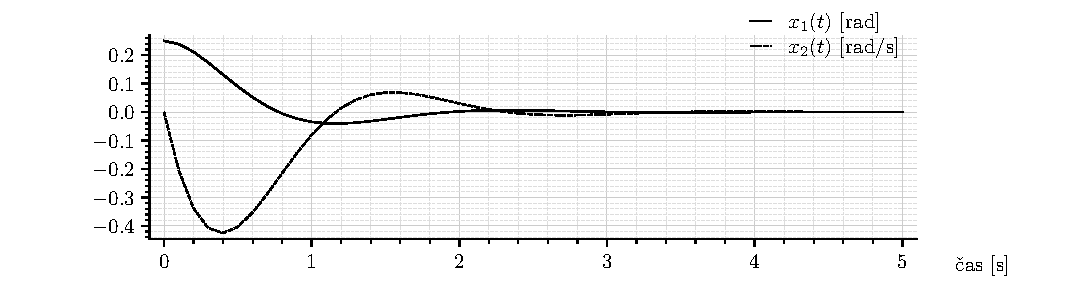
\includegraphics{cv03_fig_1.pdf}
    }

    \vspace{-4mm}

    \figcaption{Grafické zobrazenie numerického riešenia.}
    \label{cv3obr1}

    }

\end{center}

Na obr.~\ref{cv3obr1} ide však len o akési základné zobrazenie. Zmysluplnejšie by napríklad mohlo byť, ak by sme do grafu nakreslili len priebeh polohy (výchylky) kyvadla samostatne a navyše nie v radiánoch ale v stupňoch -- viď obr.~\ref{cv3obr2}. Pre takýto obrázok možno do hl. skriptu pridať:
\begin{lstlisting}[language=Matlab, title=Časť súbora hlSkript.m, name=hlSkript]
    figure(2)
    plot(t,x(:,1)*180/pi)
\end{lstlisting}

\begin{center}

    \vbox{

    \makebox[\textwidth][c]{%
    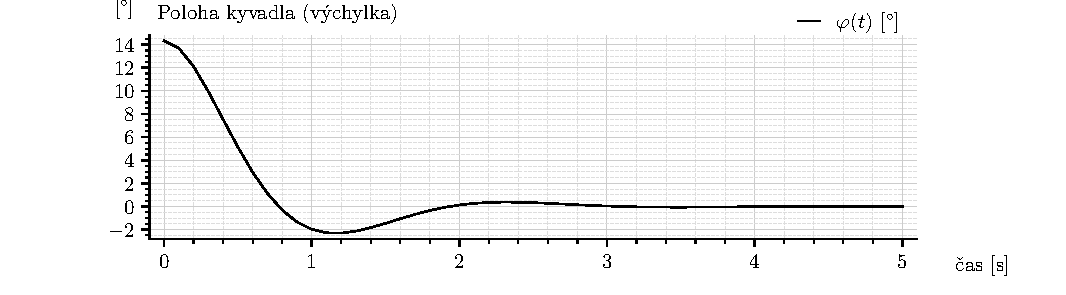
\includegraphics{cv03_fig_2.pdf}
    }

    \vspace{-4mm}

    \figcaption{Grafické zobrazenie priebehu polohy kyvadla.}
    \label{cv3obr2}

    }

\end{center}

\paragraph{Systém so vstupným signálom}

Modifikujme pôvodnú funkciu a skrip v MATLAB-e tak, aby bolo možné simulovať nenulový vstupný signál $u(t)$.

Funkciu, ktorá realizuje sústavu diferenciálnych rovníc \eqref{rovniceKyvSSpredpis} aj so vstupným signálom $u(t)$:
\begin{lstlisting}[language=Matlab, title=Celý súbor PravaStr\_u.m]
function dotx = PravaStr_u(t,x, u)

global m l g beta

dotx1 =  x(2);
dotx2 = - (beta/m*l^2)*x(2) - (g/l)*sin(x(1)) + (1/m*l^2) * u;

dotx = [dotx1; dotx2];

end
\end{lstlisting}

Vytvorme „hlavný skript“, v ktorom všetko potrebné nastavíme, a v ktorom budeme volať ODE solver:
\begin{lstlisting}[language=Matlab, title=Súbor hlSkript\_u.m]
global m l g beta

m = 1; %kg
l = 1; %m
g = 9.81; %m/s^2
beta = 2*0.5*sqrt(g/l); %kgm^2/s

u = 3

[t,x] = ode45(@(t,x) PravaStr_u(t,x,u), [0 10], [0; 0]);

figure(3)
plot(t,x(:,1)*180/pi)
\end{lstlisting}

Simulujme prípad keď napríklad $u(t) = 3$ [kg m$^2$ s$^{-2}$] (pozn.: pre lepšiu názornosť uvažujme začiatočné podmienky nulové). Výsledok simulácie je na obrázku~\ref{cv3obr4}.

\begin{center}

    \vbox{

    \makebox[\textwidth][c]{%
    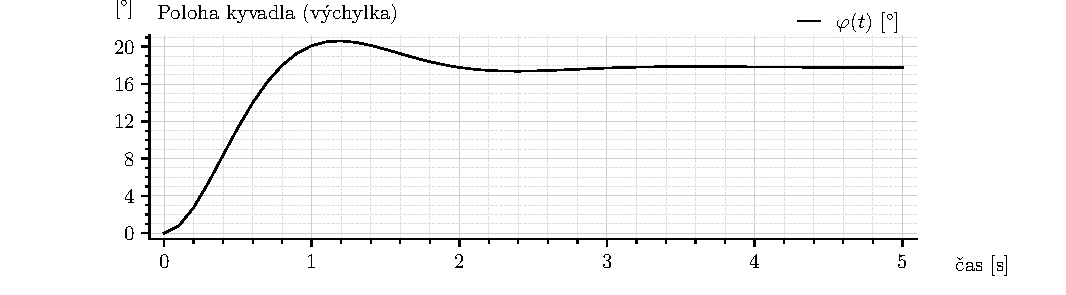
\includegraphics{cv03_fig_4.pdf}
    }

    \vspace{-4mm}

    \figcaption{Grafické zobrazenie priebehu polohy kyvadla.}
    \label{cv3obr4}

    }

\end{center}


\subsection{Python}

Nasledovne by vyzeralo hľadanie numerického riešenia v rámci jazyka Python.


Knižnica \href{https://www.scipy.org/}{\color{NavyBlue} SciPy}, presnejšie \href{https://docs.scipy.org/doc/scipy-0.18.1/reference/integrate.html}{\color{NavyBlue} scipy.integrate} obsahuje ODEsolver s názvom \verb|odeint|. Vytvorme skript využívajúci tento ODE solver:


\begin{lstlisting}[language=Python, title=Skript v Python-e]
import numpy as np
from scipy.integrate import odeint
import matplotlib.pyplot as plt

m = 1.0
l = 1.0
g = 9.81
beta = 2 * 0.5 * np.sqrt(g/l)

def fcn_rovniceKyvadla(x, t, u):
    x_1, x_2 = x
    dotx_1 = x_2
    dotx_2 = -(beta/m*l**2) * x_2 - (g/l) * np.sin(x_1) + (1.0/m*l**2) * u
    return [dotx_1, dotx_2]


timeVect = np.arange(0, 5.1, 0.1)

u = 0

x = odeint(fcn_rovniceKyvadla,
           [np.pi/4, 0],   # zaciatocne podmienky
           timeVect,
           args=(u,),
           )

plt.figure(1)
plt.plot(timeVect, x)
plt.xlabel(u'cas [s]')
plt.legend(['$x_1(t)$ [rad]', '$x_2(t)$ [rad/s]'])

plt.figure(2)
plt.plot(timeVect, x[:,0]*180/np.pi)
plt.xlabel(u'cas [s]')
plt.ylabel(u'$x_1(t)$ [stupne]')
\end{lstlisting}






















\end{document}
